\chapter{Tribal NeuroSim: játéklogika és neurális döntéshozatal}

\section{Neurális döntéshozatal és klaszter-priorok}

Minden szimulált törzs egy neurális hálózatot hordoz, amelynek felépítése a NEAT (\textit{NeuroEvolution of Augmenting Topologies}) paradigmáját követi \cite{stanleymiikkulainen2002}. A rendszer \textit{nem alkalmaz visszaterjesztést}: a törzs nem kap tanítójelet egy valódi League of Legends-meccsel kapcsolatban. Ehelyett a fitnesz a szimulációs folyamat kimenetéből következik (túlélési időből, megszerzett területből, populációméretből és elért polity-szintből), és minden ezer tickenként kerül kiértékelésre \cite{holland1992}.

Minden törzs inicializálásakor valódi meccselőzményekből levezetett klaszterszintű teljesítménymutatókat kap iniciális genomszekvenciaként: \textbf{A\_combat}, \textbf{A\_resource}, \textbf{A\_map\_objective}, \textbf{A\_risk}, \textbf{A\_team}. Az inicializálás során minden törzshöz egy \textit{Genome::new(11,~7)} struktúra jön létre 11~bemeneti csomóponttal, 7~kimeneti csomóponttal és 84~kezdeti kapcsolattal.

\section{A 11 bemeneti jel és a 7 kimeneti hajtóerő}

A genomból minden tickben következtetés indul el: a neurális hálózat 11 bemeneti jelet olvas be, és 7 kimeneti hajtóerőt ad vissza. A bemenetek egy része a törzs pillanatnyi állapotát tükrözi (élelmiszer, populáció, veszély), a másik része pedig a klaszterből örökölt, generációs határpontokon lassan mutálódó teljesítményprofil. A kimenetek közvetlenül a törzs viselkedési döntéseit modulálják: háborúindítás, terjeszkedés, szövetségkötés vagy visszavonulás.

Az \ref{tab:neurosim-inputs} táblázat a neurális hálózat 11 bemeneti jelét mutatja be, megkülönböztetve a dinamikus (tick-szintű) és az invariáns (generációs) jeleket.

\begin{table}[h]
  \centering
  \caption{A neurális hálózat 11 bemeneti jele.}
  \label{tab:neurosim-inputs}
  \begin{tabular}{|c|l|l|l|}
    \hline
    \textbf{Index} & \textbf{Változónév} & \textbf{Leírás} & \textbf{Jelleg} \\
    \hline
    0 & \textit{food\_ratio}         & Élelmiszerkészlet / populáció         & Dinamikus \\
    1 & \textit{pop\_ratio}          & Populáció / maximális kapacitás        & Dinamikus \\
    2 & \textit{territory}           & Igényelt tile-ok száma / 100           & Dinamikus \\
    3 & \textit{feed\_risk}          & Éhhalál-közelség (1{,}0 = kritikus)   & Dinamikus \\
    4 & \textit{a\_combat}           & Harci teljesítmény-artifact             & Invariáns* \\
    5 & \textit{a\_resource}         & Erőforrás/gazdaság-artifact             & Invariáns* \\
    6 & \textit{a\_map\_objective}   & Objektívkontroll-artifact               & Invariáns* \\
    7 & \textit{a\_team}             & Csapatkoordinációs artifact             & Invariáns* \\
    8 & \textit{nearest\_enemy}      & Legközelebbi ellenfél hex-távolsága    & Dinamikus \\
    9 & \textit{nearest\_ally}       & Legközelebbi szövetséges hex-távolsága & Dinamikus \\
   10 & \textit{a\_risk}             & Kockázattűrési artifact                 & Invariáns* \\
    \hline
  \end{tabular}
  \begin{flushleft}
    \small{* Csak generációs határpontokon (1000 tickenként) frissül, mutáció révén.}
  \end{flushleft}
\end{table}

Az \ref{tab:neurosim-outputs} táblázat a 7 kimeneti hajtóerőt és az aktiválási küszöbértékeket tartalmazza.

\begin{table}[h]
  \centering
  \caption{A 7 kimeneti hajtóerő és hatásuk a törzs viselkedésére.}
  \label{tab:neurosim-outputs}
  \begin{tabular}{|l|l|l|}
    \hline
    \textbf{Változónév} & \textbf{Viselkedési hatás} & \textbf{Aktiválási küszöb} \\
    \hline
    \textit{aggression}      & Háborúindítási valószínűség modulálása       & $> 0{,}45$ \\
    \textit{resource\_drive} & Területterjeszkedési prioritás                & $> 0{,}25$ \\
    \textit{goal\_drive}     & Szövetségkezdeményezés, polity-fejlesztés     & $> 0{,}55$ / $> 0{,}50$ \\
    \textit{migration\_drive}& Migráció indítása (\textit{Settling} állapotból) & $> 0{,}55$ \\
    \textit{raid\_drive}     & Opportunista háború gyengébb szomszéd ellen  & $> 0{,}35$ \\
    \textit{isolation}       & Szövetségajánlat elutasítása                 & $> 0{,}75$ \\
    \textit{expansion\_speed}& Tile-igénylési sebesség (hűtési idő módosítás) & Folytonos \\
    \hline
  \end{tabular}
\end{table}

\section{Fitness, mutáció és leszármazási öröklés}

A fitnesz öt komponensből áll: \textit{survival\_ticks}, \textit{territory}, \textit{population}, \textit{polity\_tier} és \textit{war\_record}. A mutáció minden 1000. ticknél következik be. Az alap mutációs ráta $\mu_0 = 0{,}05$; a fitnesz-rangsor alapján ez differenciált:

\begin{equation}
\mu_i =
\begin{cases}
2\mu_0 & \text{ha } r_i \leq 0{,}20 \text{ (leggyengébb 20\%)} \\
\mu_0  & \text{ha } 0{,}20 < r_i < 0{,}80 \\
\tfrac{1}{2}\mu_0 & \text{ha } r_i \geq 0{,}80 \text{ (felső 20\%)}
\end{cases}
\end{equation}

ahol $r_i \in [0,1]$ az $i$-edik törzs relatív fitnesz-rangszáma a populációban.

Fuzionálás feltétele mindkét félnél: \textit{goal\_drive}~$> 0{,}55$, egyik sem tartózkodik \textit{AtWar} állapotban, és \textit{isolation}~$< 0{,}75$. A fuzionálásból keletkező örökös genomja fitnesz-súlyozott keverék: \textit{Genome::inherit\_from(parent\_a, parent\_b, fitness\_a, fitness\_b)}.

Az első kísérleti futtatás (599 törzs, Flexset, 1200 tick) kimeneti aktivitás- és fitnesz-differenciáció adatai, valamint a liveness-fix részletei a kibővített verzió 14. fejezetében találhatók \cite{premadegraph-full}. A \ref{fig:genome-graph} ábra a klaszter-szintű teljesítménymutatókból felépített kezdeti genomszekvenciát mutatja be.

\begin{figure}[H]
\centering
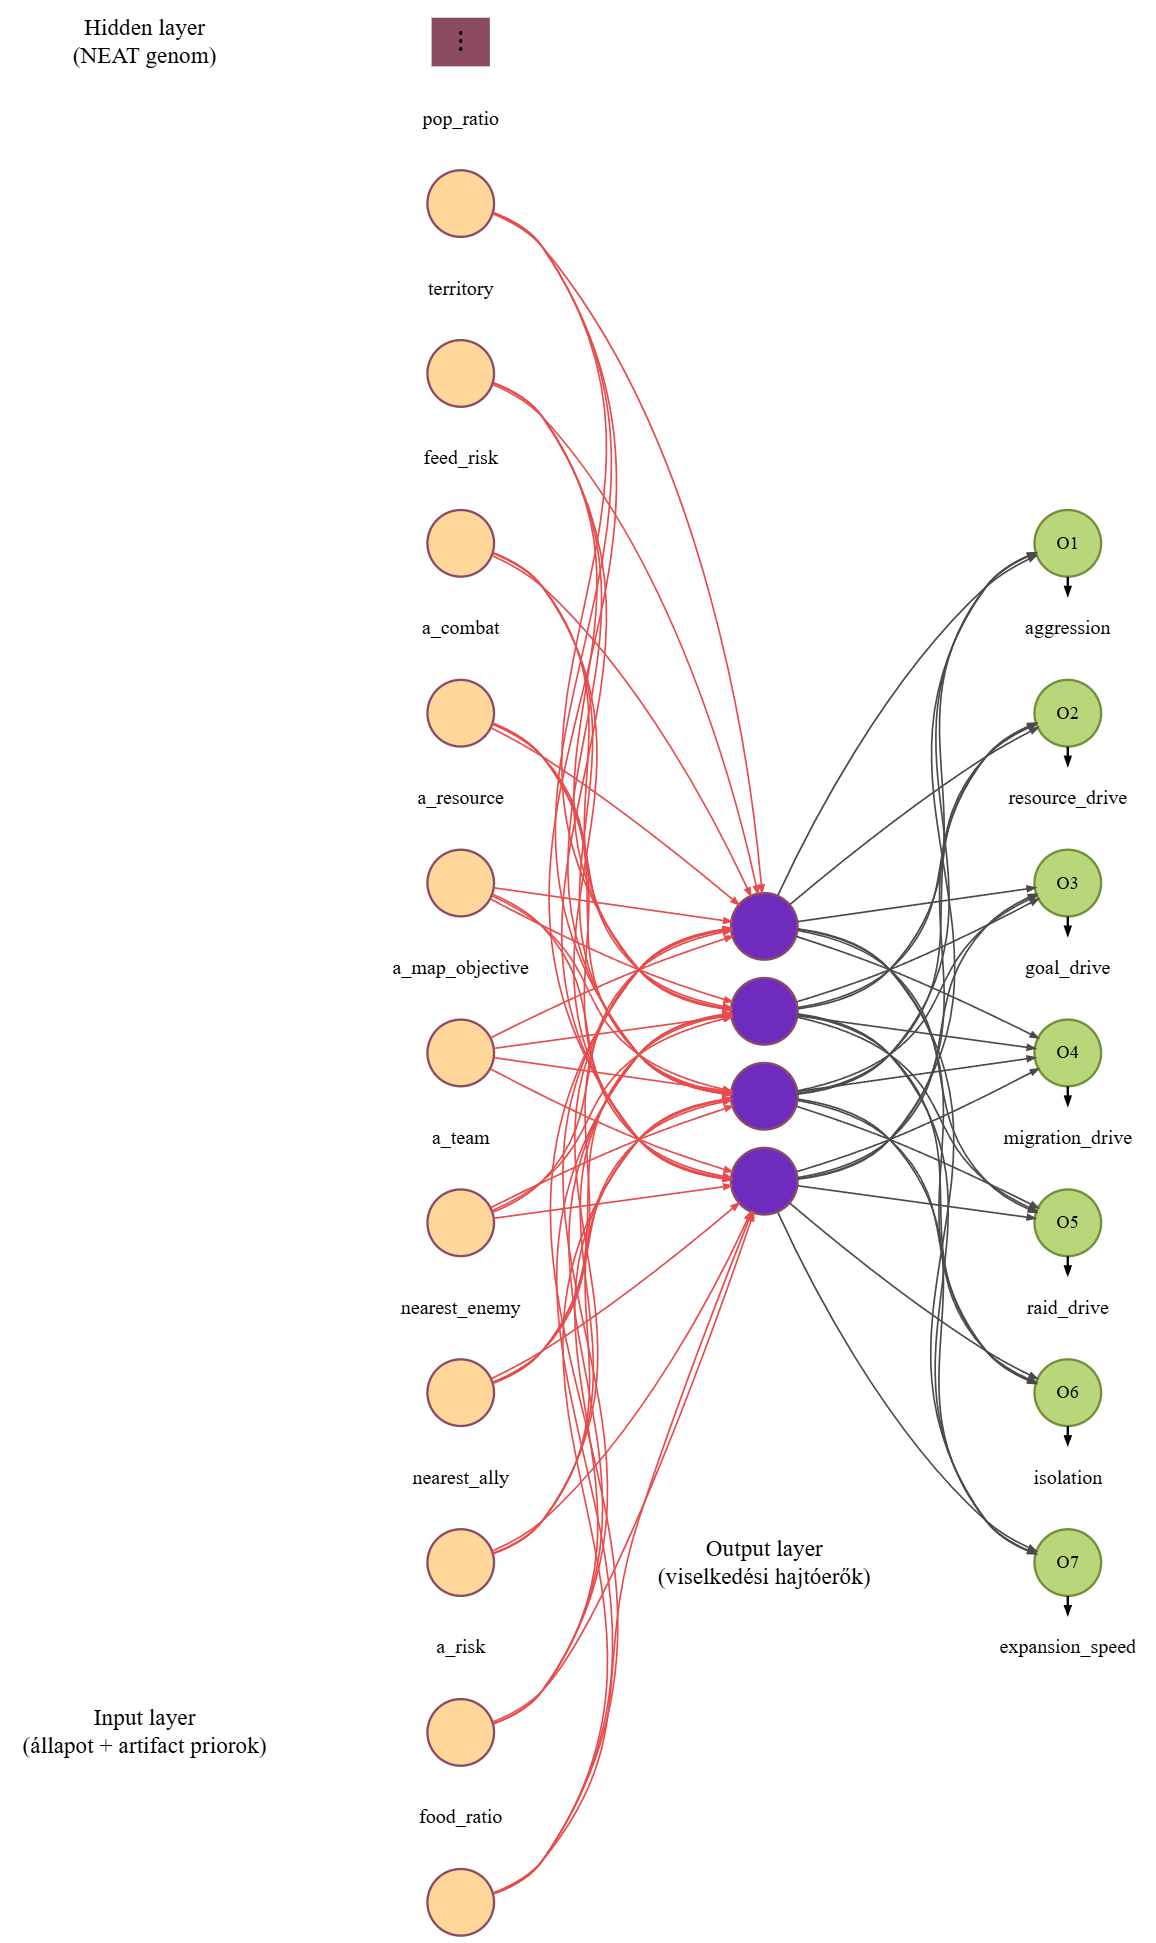
\includegraphics[width=0.90\textwidth,keepaspectratio]{assets/diagrams/genome_graph.png}
\caption{A genomgráf:  teljesítménymutatóiból felépített kezdeti genomszekvencia vizualizációja}
\label{fig:genome-graph}
\end{figure}
